\documentclass[12pt]{article}

\usepackage{times,fullpage,xspace,fancyhdr,url}
\usepackage[pdftex]{graphicx}
\usepackage[pdftex,
            a4paper,
            colorlinks=true,
            urlcolor=black,
            linkcolor=black,
            citecolor=black,
            bookmarksopen=false,
            bookmarksnumbered=true,
            pdfstartview=FitH]{hyperref}

\usepackage{graphicx}
\usepackage{xspace,color}
\pdfcompresslevel=9
\newcommand{\leaguename}{RoboCup Standard Platform League (NAO) }
\hypersetup{
 pdftitle={\leaguename Technical Challenges 2014},
 pdfauthor={Technical Committee},
}
\usepackage[latin1]{inputenc}
\usepackage{amsmath}
\usepackage{times}

% comment 'disable' in to disable all the todo notes :)
\usepackage
[
%disable
]{todonotes}

\sloppy
\newcommand{\ie}{\mbox{i.\,e.}\xspace}
\newcommand{\eg}{\mbox{e.\,g.}\xspace}
\newcommand{\cf}{\mbox{cf.}\xspace}
\newcommand{\comment}[1]{\marginpar{\pdfannot width 4in height .5in depth 8pt {/Subtype /Text /Contents (#1)}}}
\newcommand{\inparagraph}[1]{\paragraph{#1\hspace{-1em} }}

\long\def\commentk#1{{\bf ++K: #1++}}

% some colors
\definecolor{orange}{rgb}{1,0.5,0}
\definecolor{red}{rgb}{1,0,0}
\definecolor{green}{rgb}{0,1,0}


\title{\leaguename \\ Technical Challenges}
\author{RoboCup Technical Committee}
\date{(2015 technical challenge rules, as of \today)}

\setlength{\parindent}{0pt}
\setlength{\parskip}{6pt plus 6pt minus 3 pt}
\setcounter{tocdepth}{1}
\widowpenalty=10000
\clubpenalty=10000

\pagestyle{fancy}
\lhead{}
\chead{}
\rhead{}
\lfoot{}
\cfoot{}
\rfoot{}

\renewcommand{\headrulewidth}{0.4pt}
\renewcommand{\footrulewidth}{0.4pt}

% needed to align an image and text correctly side by side
\newcommand{\imagebox}[1]{\raisebox{2ex}{\raisebox{-\height}{#1}}}



\begin{document}

\maketitle

At RoboCup 2015, the Standard Platform League will hold three different technical challenges, which are described in this document.

The scores earned in each challenge will vary in magnitude.  Hence, they must be scaled before calculating the overall technical challenge rankings.  Teams who do not participate in a challenge will receive 0 points for that challenge.  The team with the highest total score for a challenge will get 25 points for that challenge, while the team with the lowest total score for a challenge will get 5 points for that challenge.  A linear equation will then be fit to these two points, and each other participating team in that challenge will gain points for that challenge based on this equation.

For all three challenges, no changes of code or configuration are allowed for any participating team after the first team starts the challenge. 

Questions or comments on these rules should be mailed to {\small \url{rc-spl-tc@lists.robocup.org}}.

\vfill

\renewcommand\contentsname{Challenges}
\tableofcontents
\setcounter{tocdepth}{1}

\thispagestyle{fancy}

\clearpage

\cfoot{\thepage}
\setcounter{page}{1}

\newcommand{\openMinNum}{three}


% % % % % % % % % % % % % % % % % % % % % % % %


\section{Corner Kicks Challenge}

\begin{figure}[t]
\centerline{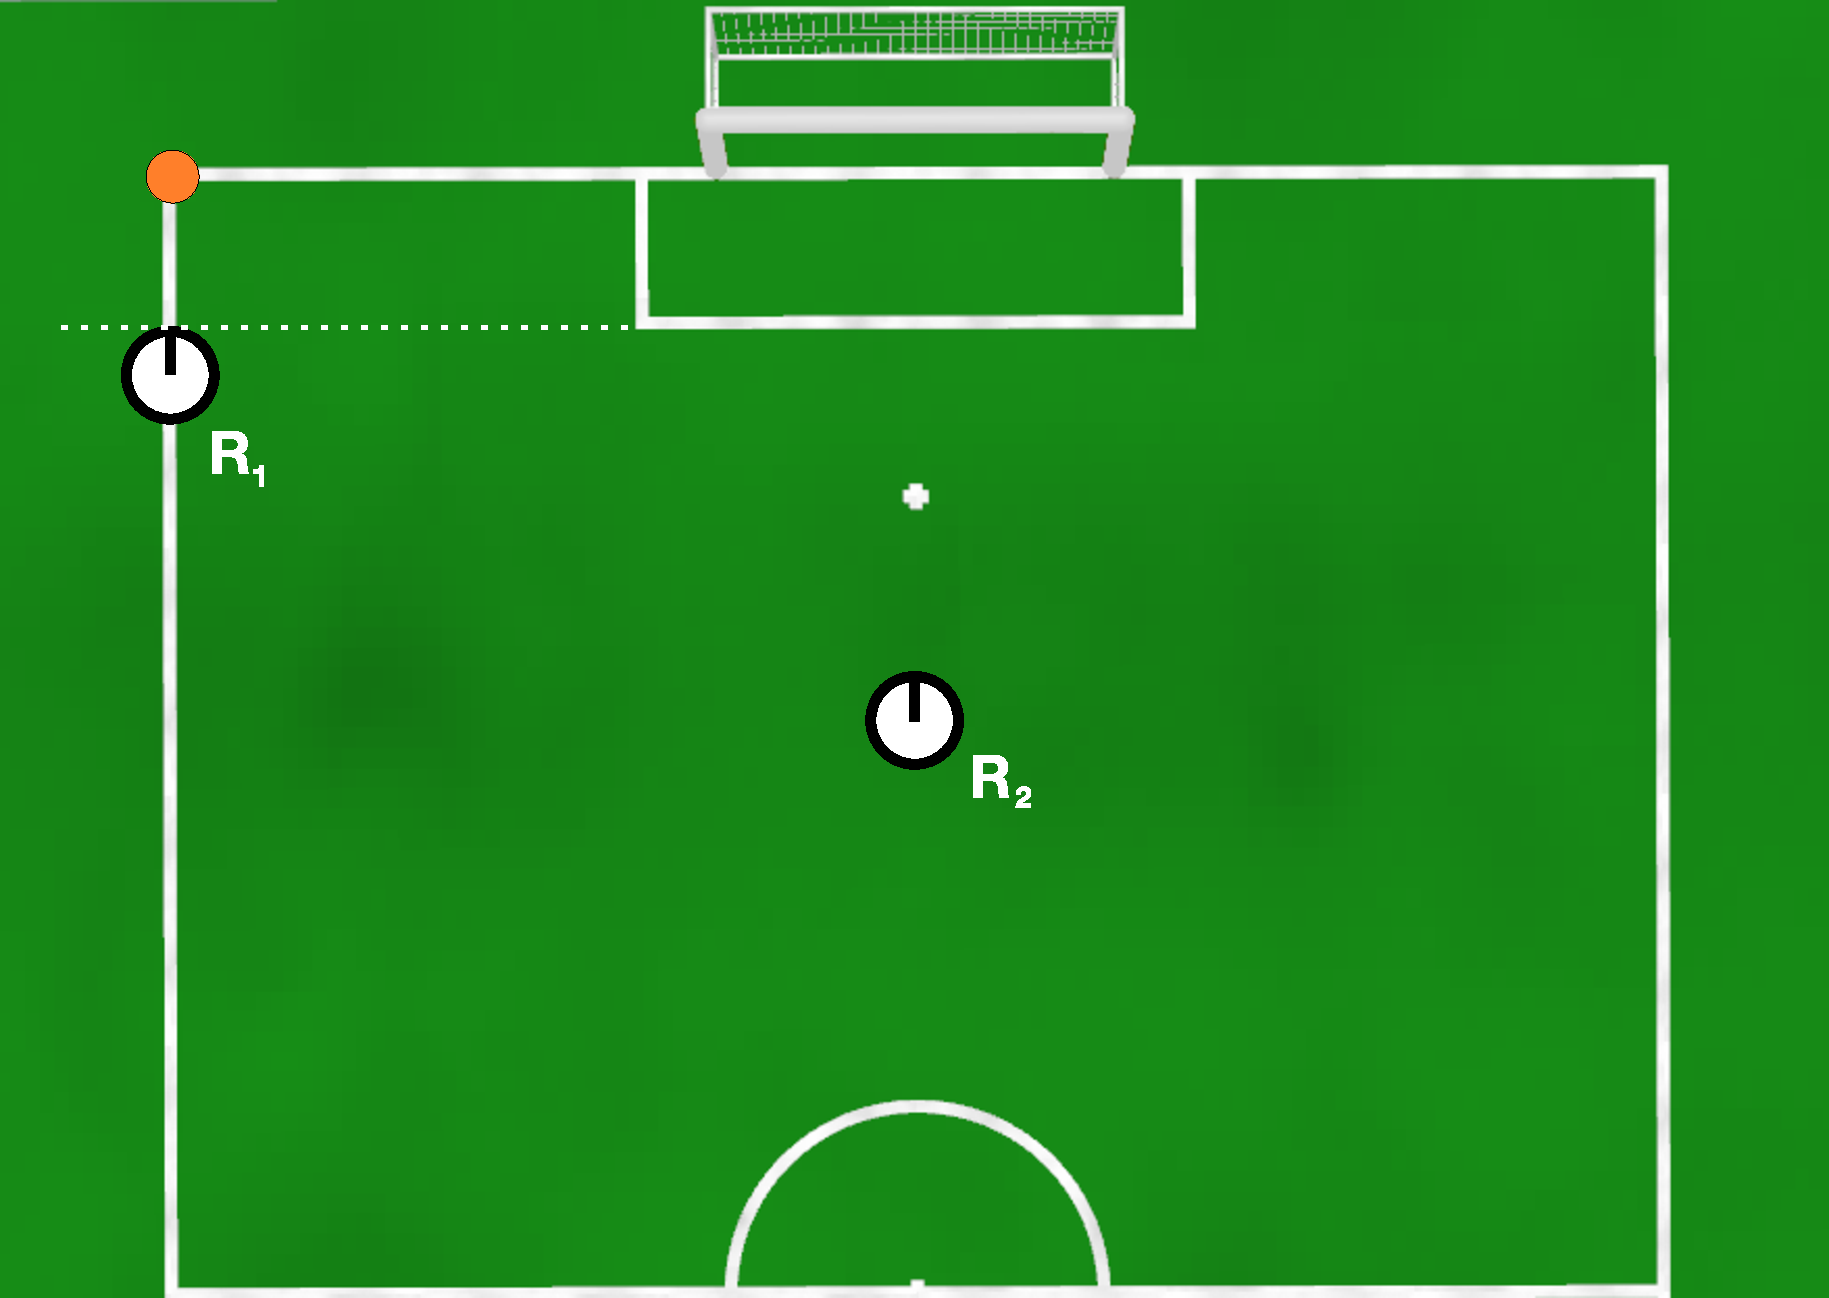
\includegraphics[width=0.8\columnwidth]{figures/corner-kicks-challenge}}
\caption{Setup before each corner kick attempt. The robot $R_1$, which has to carry out the corner kick, is placed on the sideline with its feet touching a virtual extension of the penalty area's front line. The robot $R_2$ is standing at the default penalty kick position, \ie 1 m behind the penalty mark. The ball is placed in the left corner of the field. Please note that during the challenge, several opponent robots will be placed on the field. Their positions will not be announced in advance.}
\label{fig:corner_kicks_challenge}
\end{figure}


The purpose of this challenge is to foster passing skills, team play, and the perception of opponent robots.

\subsection{Setup}
The ball is placed at one of the field corners next to one of the goals. Each participating team has to provide two robots (whose jersey color can be chosen freely, wearing no jersey is legal, too). These robots will be placed at the two predefined positions $R_1$ and $R_2$ (see Fig. \ref{fig:corner_kicks_challenge}). The initial game state is SET. Initially, there are no opponent robots. The time limit for this challenge is 3 minutes.

\subsection{Procedure}
The game state changes to PLAYING and the robots can start to carry out the corner kick. To achieve a goal, both robots need to have touched the ball. The robot at position $R_1$ has to be the first who touches the ball. There are no other restrictions regarding a minimum or maximum number of touches. If the other robot touches first, the game state changes to SET again and the corner kick is repeated. The time is stopped during this reset.

If the ball leaves the field, it is placed in the corner again. In this case, the time is not stopped and the game state does not change to SET. 

If the ball enters the goal, the game state changes to SET and the time stops. Both robots are put back on their start positions again.

After each goal, one opponent robot (standing and not moving) is added to the field to make the following corner kick attempt more difficult. The positions of the opponent robots will not be announced in advance. There will not be more than 4 opponents, i.e. after having scored four goals, the setup will remain constant. The configuration of the opponent robots will be the same for all teams. 

If an opponent becomes pushed, or a playing robots leaves the field or is fallen or holds the ball or plays the ball with its hands (everything according to the definitions in the normal rules), the game state changes to SET and the time stops. Both robots are put back on their start positions again.

\subsection{Score}
Each goal will be awarded with one point.
Before the first goal is scored, a team receives one initial point once both robots have touched the ball.

\subsection{Origin, Color, and Handling of Opponent Robots}
The opponent robots will be provided by the other teams that participate in this challenge. Whenever a team has completed the challenge, it will provide its two robots as potential opponents for the next two participating teams. The last teams participating in this challenge have to provide their robots for the first participants. The Technical Committee will announce a detailed plan in advance to the challenge.

All opponent robots must wear the cyan standard jerseys.

To avoid any unnecessary damages to the robots, the Technical Committee members that conduct this challenge can try to catch falling opponent robots and put them back in a standing position if requested by the teams.

\newpage
% % % % % % % % % % % % % % % % % % % % % % % %



\section{Many Carpets Challenge}

\subsection{Purpose}

The purpose of the challenge is the improvement of motion skills. Moreover, we intend to study whether robots are able to play on different types of carpets.

\subsection{Selection of Carpets}

Each team may bring one carpet to the competition (this is encouraged, but not required). This carpet should be approximately 3*4 meters, with no seams or lines.  It is preferable for the carpet to be significantly different than the current SPL carpet (texture, fiber height, etc). If a team brings a carpet, it will use the carpet it brought.  The Technical Committee will also pick 3 carpets out of all of the carpets brought by teams.  2 of these carpets will be chosen by the Technical Committee to be used in the challenge, and the third will be a spare.  All teams will complete with the 2 carpets chosen by the Technical Committee and their own carpet --- if this would result in only two carpets being used in the challenge, then the spare carpet will also be used.  Note that the Technical Committee may opt to use the spare carpet if otherwise two of the carpets used by a team in the challenge would be extremely similar (as would be the case if a team's carpet is extremely similar to one of carpets chosen by the Technical Committee).

The chosen carpets will be displayed to the teams about 24 hours before the challenge will take place.  We hope space will allow for teams to test on these carpets within the 24 hours before the challenge, but space constraints may not allow this.  Hence, teams should not plan on being able to test on the carpets before the challenge.

\subsection{Setup}

The challenge will happen on three different carpets that are chosen as stated above.   Each individual team requires exactly one robot for the challenge.

The carpet will be laid out as flat as possible.  One robot, one ball, and one goal are placed on the carpet. The goal will be placed near one of the edges of the carpet. The robot and the ball will be placed on set, but unannounced, positions on the carpet (these positions will be the same for all teams, but may vary from carpet to carpet).  The carpet will not be lined in any way.  The initial game state is SET.

\subsection{Procedure}

After the game state switches from SET to PLAYING, the robot should move to the ball and kick it into the goal (multiple kicks may be used to score if needed). After a goal has been obtained, or the ball leaves the carpet, or the robot commits any infringement (as defined by the normal SPL game rules), the challenge for the current carpet is finished. The time limit for each individual carpet is one minute. 

\subsection{Score}

For each carpet, 2.5 points will be awarded once a goal is scored, half a point once the robot touches the ball the first time, and half a point once the ball leaves the field on the ground line without scoring a goal. This way, a team can obtain at maximum of 3 points per carpet (0.5 points for touching the ball and 2.5 points for obtaining a goal).

\newpage



% % % % % % % % % % % % % % % % % % % % % % % %



\section{Realistic Ball Challenge}

The most common techniques for ball detection in the SPL mostly rely on color information. However, in accordance with the new white goals, it is expected that a more realistic ball will be adopted by the SPL in the near future.  The Humanoid Kid Size league has adopted a realistic FIFA size 1 ball that is at least 50\% white for the 2015 competitions.  Therefore, the aim of this challenge is to test whether NAO robots can detect balls other than the orange ones on the field and manipulate them as precisely as an orange ball.  Note that a similar challenge was held in the SPL in 2009, but with the majority of teams not being able to score goals with the non-orange balls.  Hence, we hold a similar challenge in 2015 to see if teams will be able to perform better with non-orange balls six years later.

\subsection{Selection of Balls}

Each team must bring one ball that is not orange or red.  It is preferable for the ball to be a realistic soccer ball in some manner (color, design, material, etc). Each team will play with the ball it brought.  The Technical Committee will also pick 5 balls out of all of the balls brought by teams.  4 of these balls will be chosen by the Technical Committee to be used in the challenge, and the fifth will be a spare.  All teams will complete with the 4 balls chosen by the Technical Committee and their own ball --- if this would result in only four balls being used in the challenge, then the spare ball will also be used.  Note that the Technical Committee may opt to use the spare ball if otherwise two of the ball used by a team in the challenge would be extremely similar (as would be the case if a team's ball is extremely similar to one of the balls chosen by the Technical Committee) or if the Technical Committee believes the ball brought by the team is orange or red.

\subsection{Setup}

The robot will start from the intersection of one of the side lines and the center line, facing towards the center of the field. The initial game state is SET. All five balls will be placed randomly within an imaginary $4m \times 4m$ area located at the center of the field at the beginning of the challenge.  There will also be two stationary robots in the  $4m \times 4m$ area that may wear any jersey that the Technical Committee choses. The purpose of placing those extra robots on the field is to make sure that there are some \emph{non-ball} objects on the field. The balls and the robots will be placed in the same positions for all teams.

\subsection{Procedure}

Once the state is switched to PLAYING, the robot has 3 minutes to detect the balls, walk towards them, and try to score as many goals as it can. The robot may attempt to score on either goal.  Normal SPL rules will be followed except in the following cases.  First, balls that go out of bounds or into the goal will be removed from the field. Second, in the case of any penalty (fallen robot, leaving the field, pushing) the clock will be stopped, the state will set switched to SET, the robot will be repositioned to the intersection of one of the side lines and the center line (facing towards the center of the field), and then the clock will be restarted and the state will be switched to PLAYING.

\subsection{Scoring}
The robot will be awarded 1 point the first time it touches each ball {\bf and} this touch moves the ball towards the goal (towards the goal is defined to be within a 90 degree cone pointing directly from the robot towards the goal).  The robot is awarded 3 points for each goal scored.  If the robot is able to score with all five balls before the time is over, then the stopwatch will be stopped, time spent for scoring will be recorded, and the robot will be awarded a additional ($\frac{180 - \emph{spentTime}}{5}$) points (where $180$ is 3 minutes in seconds and $\emph{spentTime}$ is recorded in seconds).

\end{document}

